\section{Diseño de interfaces}
\label{sec:diseno}

\subsection{Sistema de diseño}
Antes de dibujar pantallas se fijaron las reglas visuales para que todas se vean como una sola aplicación (tabla~\ref{tab:sistema}).

\begin{table}[H]
	\centering\footnotesize
	\begin{tabularx}{\textwidth}{|p{3.2cm}|X|}
		\hline
		\rowcolor{tablebackground}\color{white}\textbf{Elemento} & \color{white}\textbf{Decisión}\\
		\hline
		Tema & Material 3 con \texttt{ColorScheme.fromSeed} y color semilla guinda (\texttt{\#8C1D2F}), cercano a los colores de la universidad; los demás tonos salen del esquema. \\\hline
		Estados de ocupación & Disponible (verde), casi lleno (ámbar, desde 85\,\%) y lleno (rojo, sin cupos). Siempre con icono y texto, no solo color. \\\hline
		Espaciado & Múltiplos de 4\,dp; márgenes de pantalla de 16\,dp; separación entre tarjetas de 8 a 12\,dp. \\\hline
		Formas & Esquinas redondeadas de 12 a 20\,dp en tarjetas y avisos; botones del tema. \\\hline
		Jerarquía de texto & Estilos del tema (\texttt{titleLarge}, \texttt{titleMedium}, \texttt{bodyMedium}, \texttt{bodySmall}); títulos en negrita. \\\hline
		Objetivos táctiles & Botones principales de 48\,dp de alto. \\\hline
		Componentes propios & \texttt{CupoBar}, \texttt{EstadoChip}, \texttt{StatTile}, \texttt{Aviso}, \texttt{EstadoVacio}, \texttt{ContenidoCentrado}. \\\hline
	\end{tabularx}
	\caption{Sistema de diseño de MatrLab.}
	\label{tab:sistema}
\end{table}

\subsection{Mapa de navegación}
La aplicación tiene un solo nivel de pestañas (dentro de \texttt{ShellScreen}) y un flujo de pantallas apiladas para matricularse (figura~\ref{fig:nav}). El administrador ve las pestañas Cursos y Panel; el estudiante, Cursos, Mi horario y Alertas.

\onefig{img/d_navegacion.png}{1.0}{Mapa de navegación de MatrLab.}{fig:nav}

\subsection{Mockups}
\label{sec:mockups}
Los mockups se dibujaron antes de programar, a escala de teléfono (360\,$\times$\,740\,dp), como wireframes de mediana fidelidad. Cada número rojo identifica un elemento y la tabla contigua indica \textbf{con qué widget de Flutter se construye}, que es lo que pide la guía para explicar el mockup.


\FloatBarrier
\subsubsection*{Pantalla de inicio de sesión}
Estructura: \texttt{Scaffold} $\rightarrow$ \texttt{SafeArea} $\rightarrow$ \texttt{Center} $\rightarrow$ \texttt{SingleChildScrollView} $\rightarrow$ \texttt{ConstrainedBox(maxWidth: 420)} $\rightarrow$ \texttt{Form} $\rightarrow$ \texttt{Column(stretch)}. El \texttt{ConstrainedBox} evita que el formulario se estire en pantallas anchas y el scroll evita desbordes cuando aparece el teclado.

\begin{figure}[H]\centering
\begin{minipage}[c]{0.36\textwidth}\centering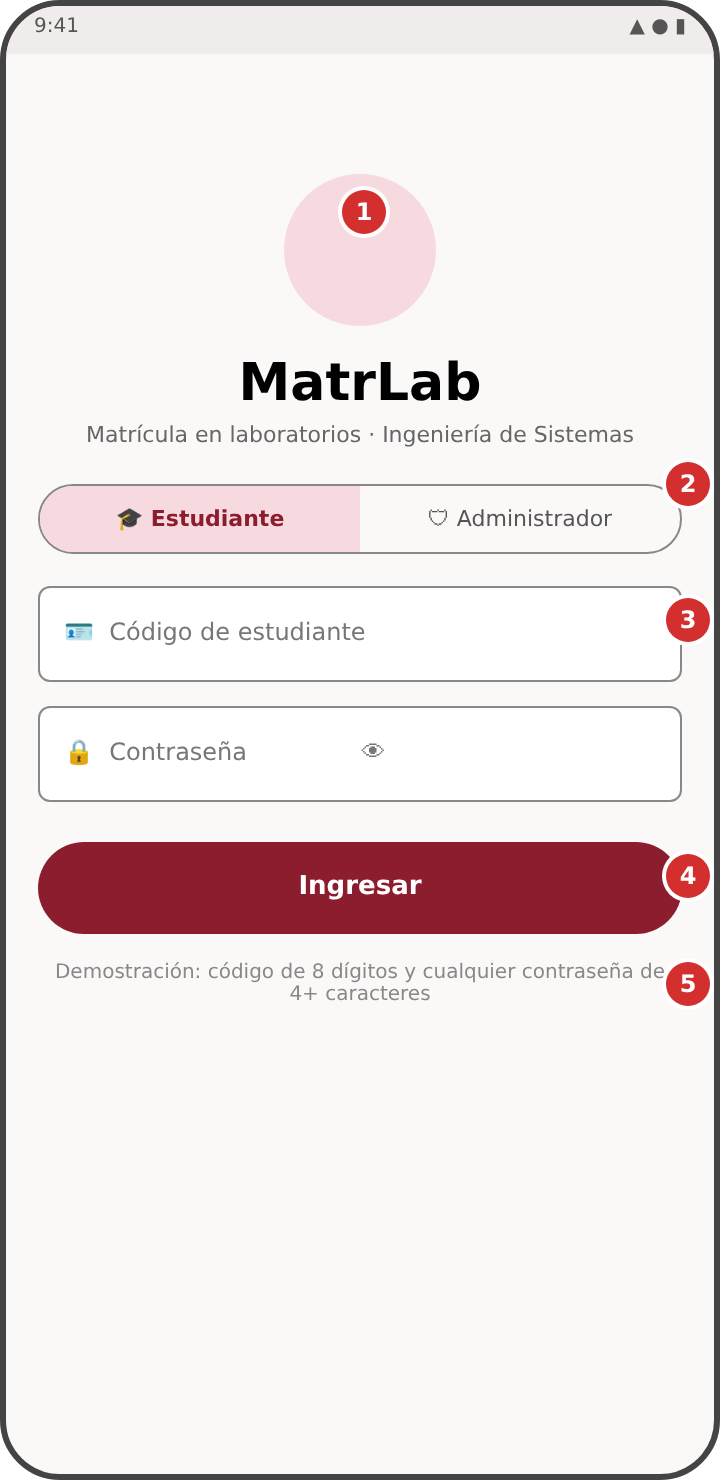
\includegraphics[width=\linewidth]{img/m01_login.png}\end{minipage}\hfill
\begin{minipage}[c]{0.60\textwidth}\footnotesize\begin{tabularx}{\linewidth}{|c|p{2.3cm}|X|}\hline\rowcolor{tablebackground}\color{white}\textbf{N.°} & \color{white}\textbf{Elemento} & \color{white}\textbf{Widget}\\\hline
1 & Logo circular & \texttt{Container} (\texttt{BoxDecoration} circular) con \texttt{Icon}, dentro de \texttt{Center} \\\hline
2 & Selector de rol & \texttt{SegmentedButton<Rol>} \\\hline
3 & Código y contraseña & \texttt{TextFormField} $\times$2 con \texttt{validator}; el segundo con \texttt{IconButton} para mostrar u ocultar \\\hline
4 & Botón Ingresar & \texttt{FilledButton} \\\hline
5 & Nota de demostración & \texttt{Text} con estilo \texttt{bodySmall} \\\hline
\end{tabularx}\end{minipage}
\caption{Mockup: Pantalla de inicio de sesión.}\label{fig:m01}\end{figure}


\FloatBarrier
\subsubsection*{Pestaña Cursos (inicio)}
Estructura: \texttt{Column} con \texttt{Padding}+\texttt{SearchBar}, \texttt{Row} de tres \texttt{Expanded}, \texttt{Wrap} de filtros y un \texttt{Expanded} que contiene el \texttt{GridView.builder} de tarjetas (no numerado). Cada tarjeta es \texttt{Card} $\rightarrow$ \texttt{InkWell} $\rightarrow$ \texttt{Padding} $\rightarrow$ \texttt{Row}[icono, \texttt{Expanded}(\texttt{Column})].

\begin{figure}[H]\centering
\begin{minipage}[c]{0.36\textwidth}\centering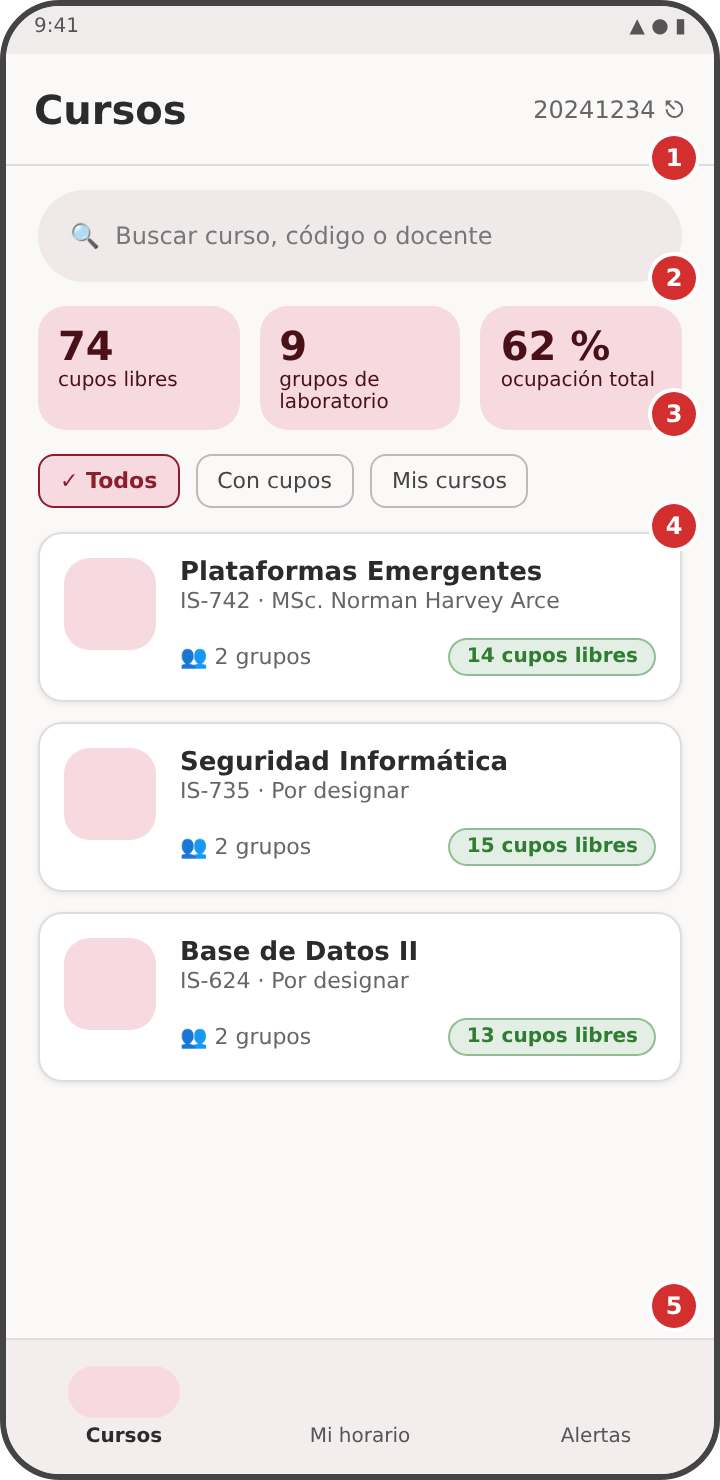
\includegraphics[width=\linewidth]{img/m02_cursos.png}\end{minipage}\hfill
\begin{minipage}[c]{0.60\textwidth}\footnotesize\begin{tabularx}{\linewidth}{|c|p{2.3cm}|X|}\hline\rowcolor{tablebackground}\color{white}\textbf{N.°} & \color{white}\textbf{Elemento} & \color{white}\textbf{Widget}\\\hline
1 & Título y cierre de sesión & \texttt{AppBar} con \texttt{actions} (\texttt{Text} + \texttt{IconButton}) \\\hline
2 & Búsqueda & \texttt{SearchBar} \\\hline
3 & Tres resúmenes & \texttt{Row} con 3 \texttt{Expanded(StatTile)} \\\hline
4 & Filtros & \texttt{Wrap} de \texttt{FilterChip} \\\hline
5 & Navegación & \texttt{NavigationBar} (con \texttt{Badge} en Alertas) \\\hline
\end{tabularx}\end{minipage}
\caption{Mockup: Pestaña Cursos (inicio).}\label{fig:m02}\end{figure}


\FloatBarrier
\subsubsection*{Detalle de un curso}
Estructura: \texttt{ListView} con \texttt{padding} de 16\,dp; la cabecera es \texttt{ClipRRect} $\rightarrow$ \texttt{Container}(degradado) $\rightarrow$ \texttt{Stack}[\texttt{Positioned}(icono), \texttt{Padding}(\texttt{Column})]. Los grupos se generan con un \texttt{for} dentro de \texttt{children}.

\begin{figure}[H]\centering
\begin{minipage}[c]{0.36\textwidth}\centering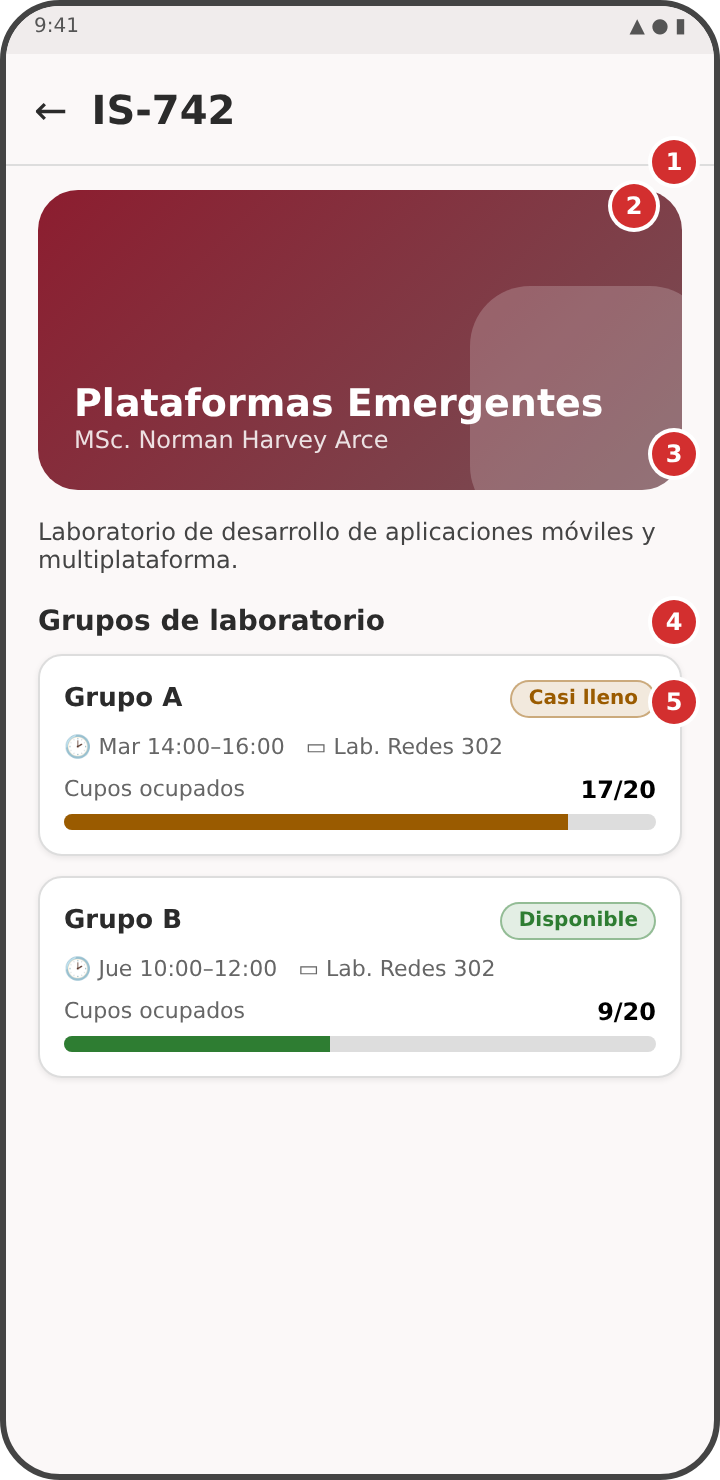
\includegraphics[width=\linewidth]{img/m03_curso.png}\end{minipage}\hfill
\begin{minipage}[c]{0.60\textwidth}\footnotesize\begin{tabularx}{\linewidth}{|c|p{2.3cm}|X|}\hline\rowcolor{tablebackground}\color{white}\textbf{N.°} & \color{white}\textbf{Elemento} & \color{white}\textbf{Widget}\\\hline
1 & Barra con flecha de regreso & \texttt{AppBar} (la flecha la agrega \texttt{Navigator}) \\\hline
2 & Cabecera con degradado & \texttt{Stack} + \texttt{Positioned}: el icono decorativo se superpone al texto \\\hline
3 & Descripción & \texttt{Text} \\\hline
4 & Tarjeta de grupo & \texttt{Card} $\rightarrow$ \texttt{InkWell} $\rightarrow$ \texttt{Column}; título y estado en una \texttt{Row} \\\hline
5 & Barra de cupos & \texttt{CupoBar}: \texttt{Column}[\texttt{Row}, \texttt{ClipRRect}(\texttt{LinearProgressIndicator})] \\\hline
\end{tabularx}\end{minipage}
\caption{Mockup: Detalle de un curso.}\label{fig:m03}\end{figure}


\FloatBarrier
\subsubsection*{Detalle de un grupo}
Estructura: \texttt{Scaffold} con \texttt{ListView} en el cuerpo y el botón de acción fijo en \texttt{bottomNavigationBar}, para que siempre esté al alcance del pulgar. El botón cambia según el caso: \emph{Matricularme}, \emph{Cancelar matrícula}, \emph{Unirme a la lista de espera} o deshabilitado (cruce de horario, curso ya matriculado).

\begin{figure}[H]\centering
\begin{minipage}[c]{0.36\textwidth}\centering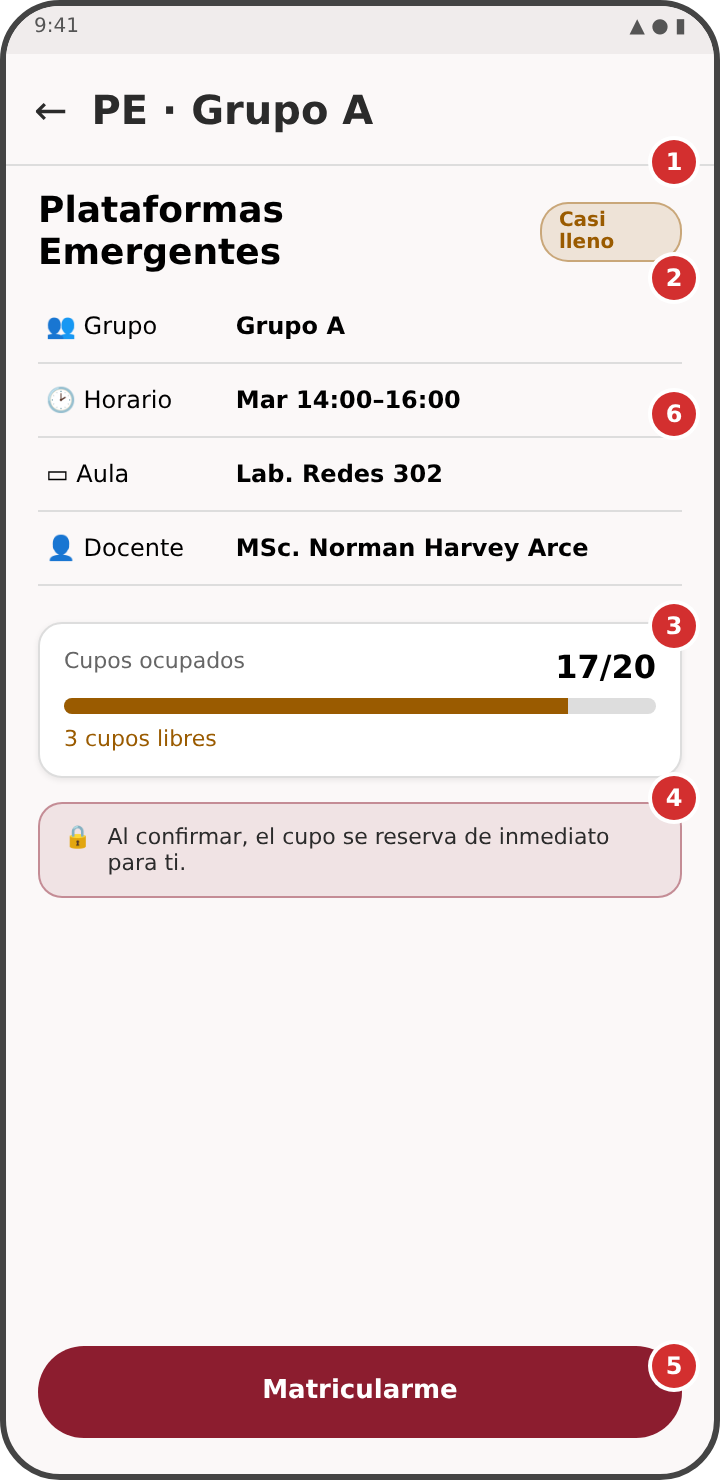
\includegraphics[width=\linewidth]{img/m04_grupo.png}\end{minipage}\hfill
\begin{minipage}[c]{0.60\textwidth}\footnotesize\begin{tabularx}{\linewidth}{|c|p{2.3cm}|X|}\hline\rowcolor{tablebackground}\color{white}\textbf{N.°} & \color{white}\textbf{Elemento} & \color{white}\textbf{Widget}\\\hline
1 & Barra superior & \texttt{AppBar} \\\hline
2 & Título y estado & \texttt{Row}[\texttt{Expanded}(\texttt{Text}), \texttt{EstadoChip}] \\\hline
6 & Datos del grupo & \texttt{Table} con \texttt{FixedColumnWidth(124)} y \texttt{FlexColumnWidth}; una \texttt{TableRow} por dato \\\hline
3 & Cupos & \texttt{Card} $\rightarrow$ \texttt{Padding} $\rightarrow$ \texttt{CupoBar(grande: true)} \\\hline
4 & Aviso contextual & \texttt{Aviso}: \texttt{Container} $\rightarrow$ \texttt{Row}[\texttt{Icon}, \texttt{Expanded}(\texttt{Text})] \\\hline
5 & Botón de acción & \texttt{SafeArea} $\rightarrow$ \texttt{Padding} $\rightarrow$ \texttt{SizedBox(48\,dp)} $\rightarrow$ \texttt{FilledButton} \\\hline
\end{tabularx}\end{minipage}
\caption{Mockup: Detalle de un grupo.}\label{fig:m04}\end{figure}


\FloatBarrier
\subsubsection*{Hoja de confirmación de matrícula}
Se abre con \texttt{showModalBottomSheet} sobre el detalle del grupo. Resume la elección antes de reservar el cupo, de modo que una pulsación accidental no matricule.

\begin{figure}[H]\centering
\begin{minipage}[c]{0.36\textwidth}\centering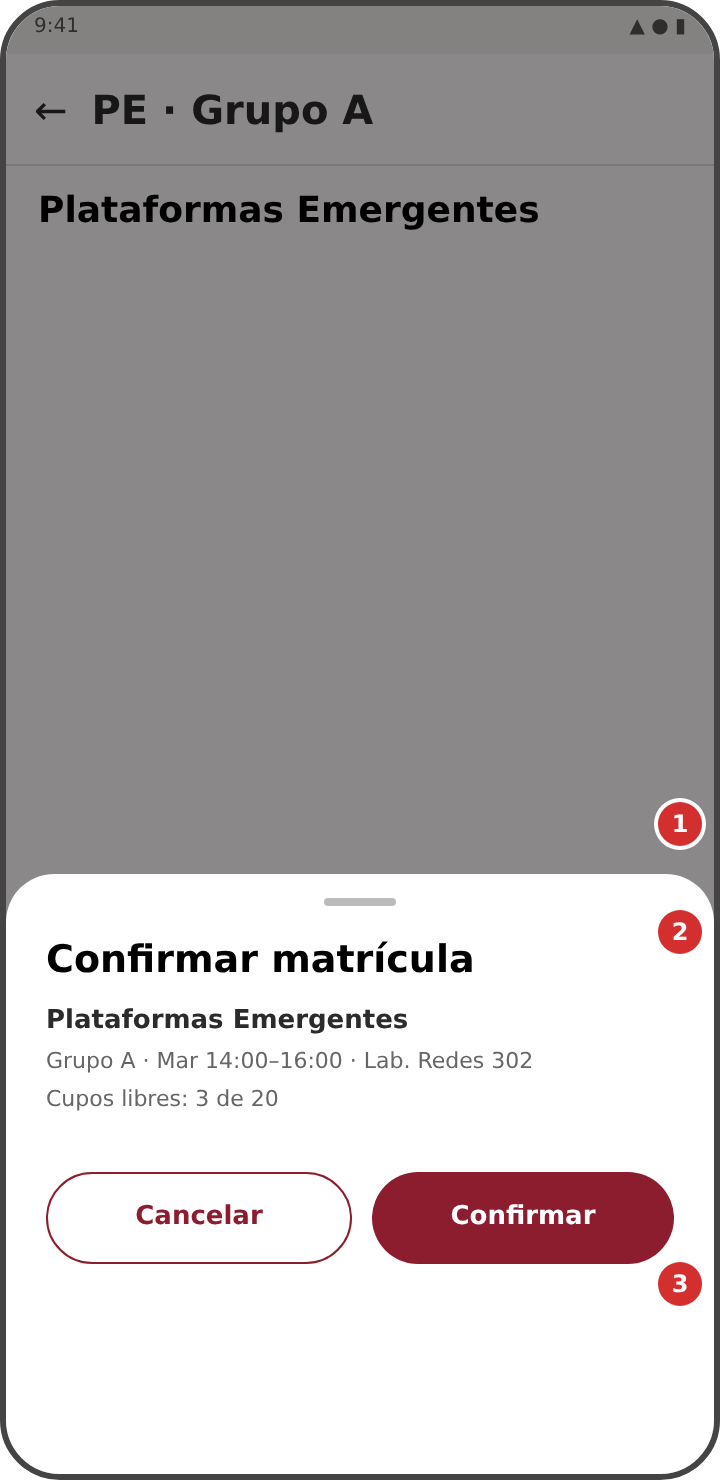
\includegraphics[width=\linewidth]{img/m05_confirmar.png}\end{minipage}\hfill
\begin{minipage}[c]{0.60\textwidth}\footnotesize\begin{tabularx}{\linewidth}{|c|p{2.3cm}|X|}\hline\rowcolor{tablebackground}\color{white}\textbf{N.°} & \color{white}\textbf{Elemento} & \color{white}\textbf{Widget}\\\hline
1 & Fondo atenuado & Barrera modal del \texttt{BottomSheet} \\\hline
2 & Hoja inferior & \texttt{SafeArea} $\rightarrow$ \texttt{Padding} $\rightarrow$ \texttt{Column(mainAxisSize: min)}, con \texttt{showDragHandle} \\\hline
3 & Cancelar / Confirmar & \texttt{Row}[\texttt{Expanded}(\texttt{OutlinedButton}), \texttt{Expanded}(\texttt{FilledButton})] \\\hline
\end{tabularx}\end{minipage}
\caption{Mockup: Hoja de confirmación de matrícula.}\label{fig:m05}\end{figure}


\FloatBarrier
\subsubsection*{Matrícula confirmada}
Estructura: \texttt{Center} $\rightarrow$ \texttt{SingleChildScrollView} $\rightarrow$ \texttt{ConstrainedBox(440)} $\rightarrow$ \texttt{Column(min)}. Los botones llevan a la pestaña Mi horario o al inicio con \texttt{popUntil}.

\begin{figure}[H]\centering
\begin{minipage}[c]{0.36\textwidth}\centering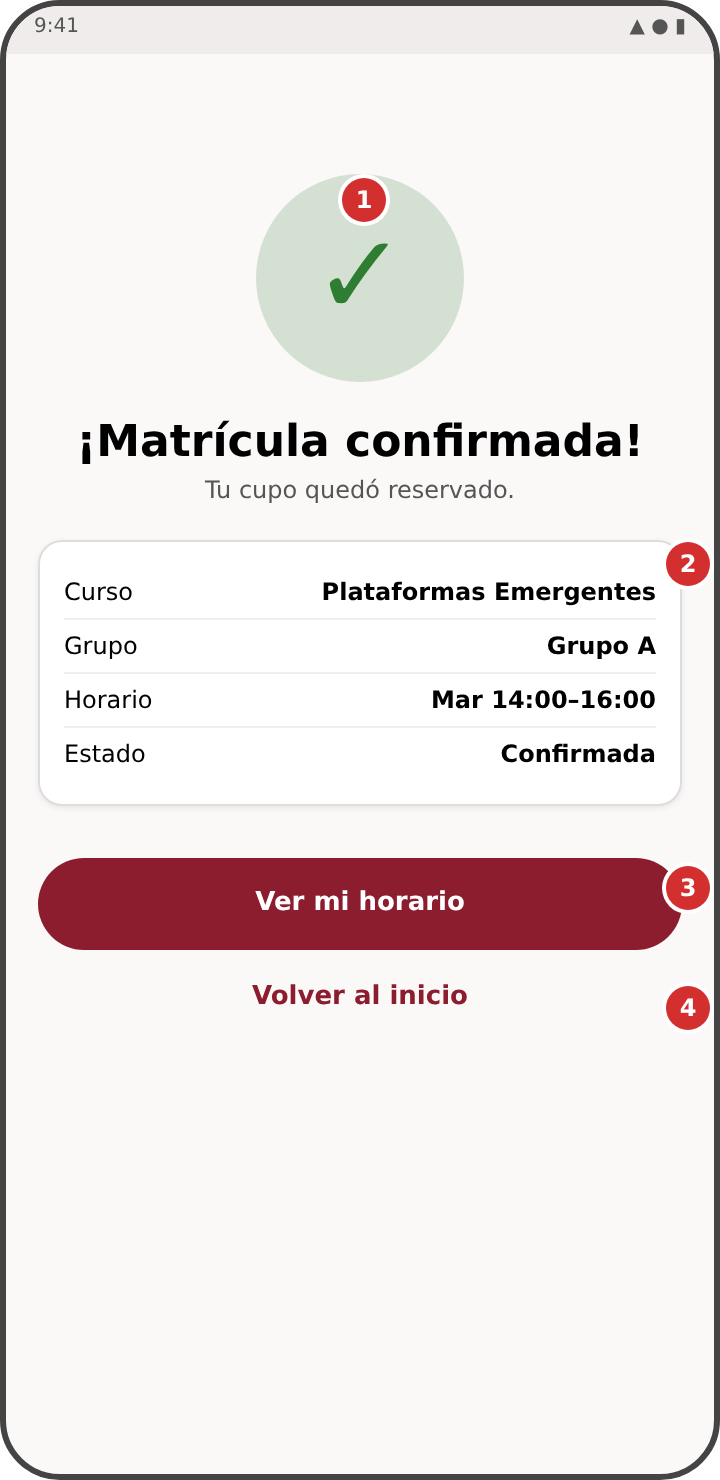
\includegraphics[width=\linewidth]{img/m06_confirmacion.png}\end{minipage}\hfill
\begin{minipage}[c]{0.60\textwidth}\footnotesize\begin{tabularx}{\linewidth}{|c|p{2.3cm}|X|}\hline\rowcolor{tablebackground}\color{white}\textbf{N.°} & \color{white}\textbf{Elemento} & \color{white}\textbf{Widget}\\\hline
1 & Icono de éxito & \texttt{Container} circular con \texttt{Icon} verde \\\hline
2 & Resumen & \texttt{Card} con \texttt{Column} de filas (\texttt{Row} + \texttt{Expanded} flex 2:3) separadas por \texttt{Divider} \\\hline
3 & Ver mi horario & \texttt{FilledButton} \\\hline
4 & Volver al inicio & \texttt{TextButton} \\\hline
\end{tabularx}\end{minipage}
\caption{Mockup: Matrícula confirmada.}\label{fig:m06}\end{figure}


\FloatBarrier
\subsubsection*{Pestaña Mi horario}
El horario semanal es una \texttt{Table} de 6 columnas (la primera de 46\,dp) y 6 filas (cabecera + cinco franjas de 2 h). Cada celda ocupada pinta la sigla del curso en un \texttt{Container} con esquinas redondeadas.

\begin{figure}[H]\centering
\begin{minipage}[c]{0.36\textwidth}\centering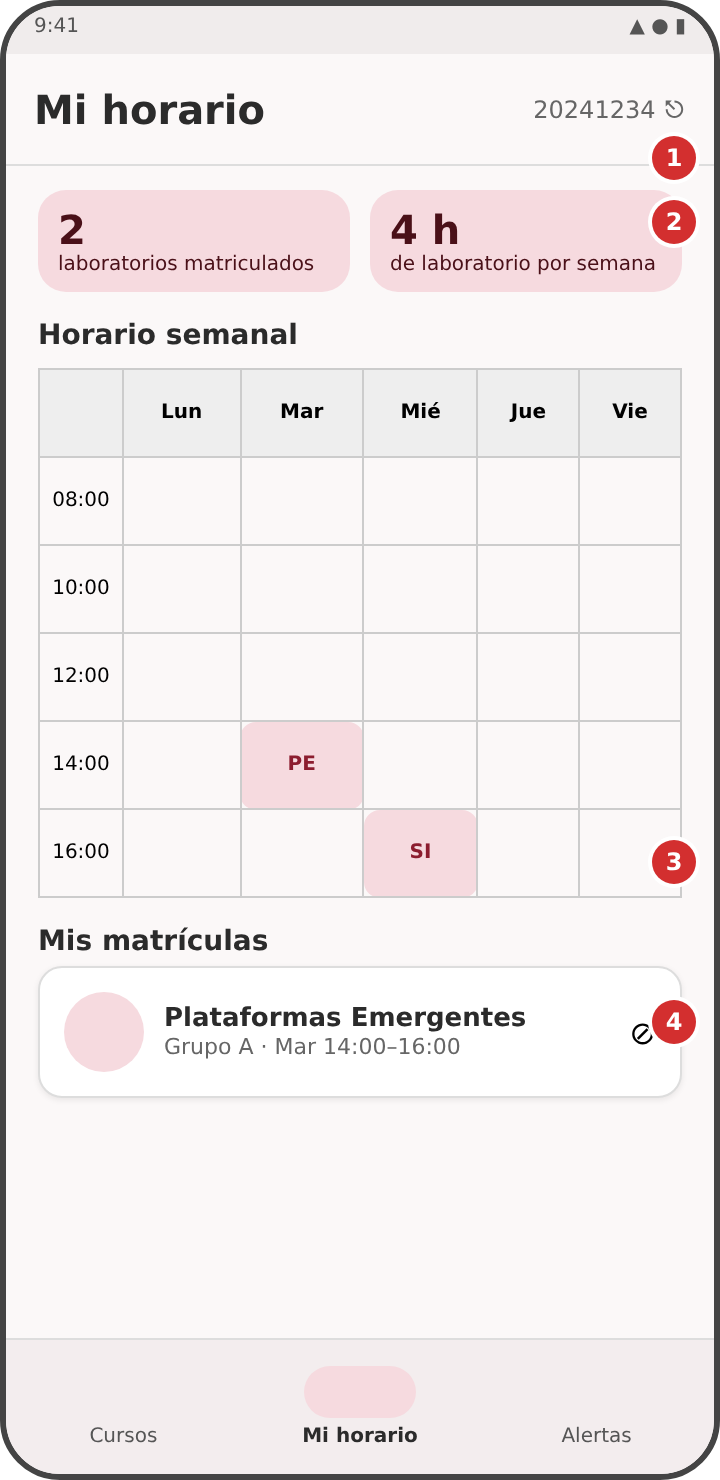
\includegraphics[width=\linewidth]{img/m07_horario.png}\end{minipage}\hfill
\begin{minipage}[c]{0.60\textwidth}\footnotesize\begin{tabularx}{\linewidth}{|c|p{2.3cm}|X|}\hline\rowcolor{tablebackground}\color{white}\textbf{N.°} & \color{white}\textbf{Elemento} & \color{white}\textbf{Widget}\\\hline
1 & Barra superior & \texttt{AppBar} \\\hline
2 & Resúmenes & \texttt{Row} con 2 \texttt{Expanded(StatTile)} \\\hline
3 & Horario semanal & \texttt{Table} con \texttt{TableBorder.all} y \texttt{FixedColumnWidth} \\\hline
4 & Mis matrículas & \texttt{Card} $\rightarrow$ \texttt{ListTile} (\texttt{leading} \texttt{CircleAvatar}, \texttt{trailing} \texttt{IconButton}) \\\hline
\end{tabularx}\end{minipage}
\caption{Mockup: Pestaña Mi horario.}\label{fig:m07}\end{figure}


\FloatBarrier
\subsubsection*{Pestaña Alertas}
Si el estudiante tiene grupos en lista de espera, se muestran como \texttt{Chip}. El punto de «no leída» es un \texttt{Badge} sin etiqueta sobre el avatar.

\begin{figure}[H]\centering
\begin{minipage}[c]{0.36\textwidth}\centering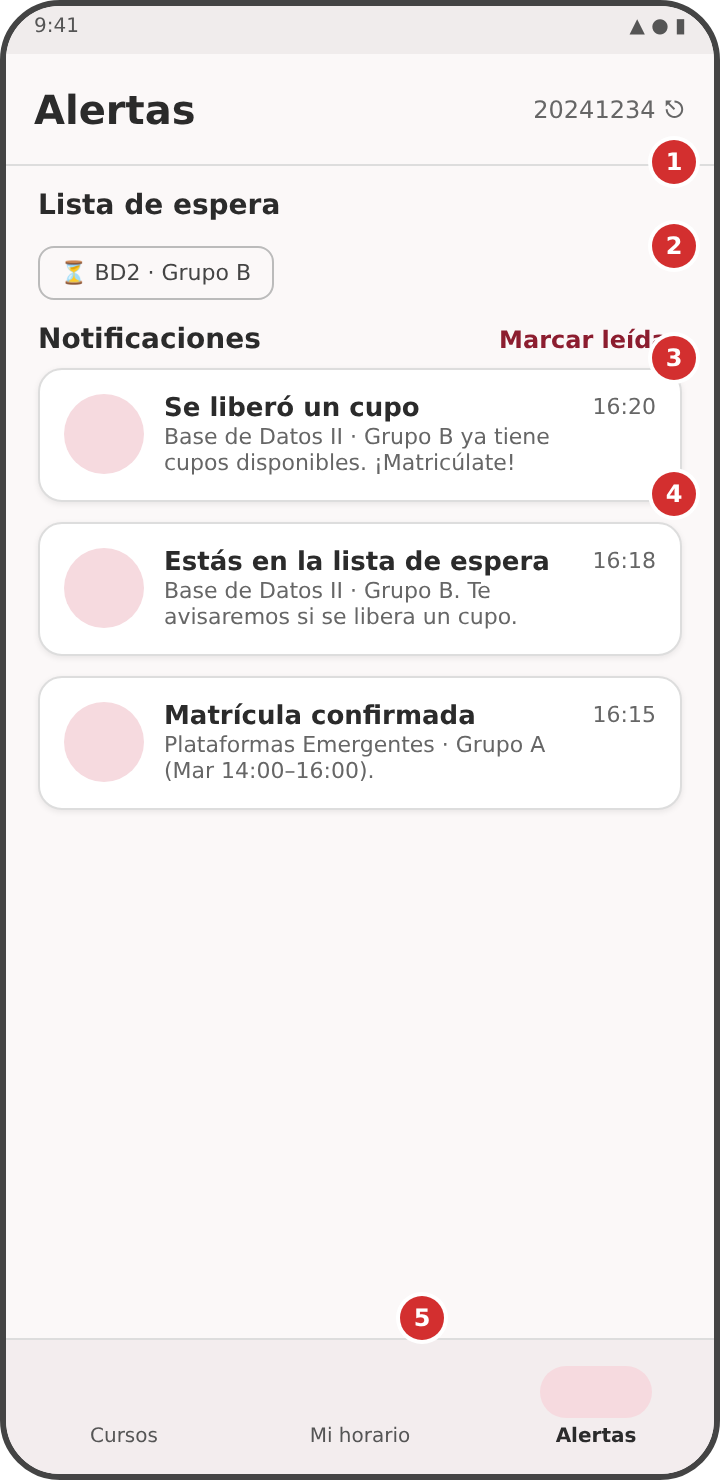
\includegraphics[width=\linewidth]{img/m08_alertas.png}\end{minipage}\hfill
\begin{minipage}[c]{0.60\textwidth}\footnotesize\begin{tabularx}{\linewidth}{|c|p{2.3cm}|X|}\hline\rowcolor{tablebackground}\color{white}\textbf{N.°} & \color{white}\textbf{Elemento} & \color{white}\textbf{Widget}\\\hline
1 & Barra superior & \texttt{AppBar} \\\hline
2 & Lista de espera & \texttt{Wrap} de \texttt{Chip} \\\hline
3 & Encabezado de notificaciones & \texttt{Row}[\texttt{Expanded}(\texttt{Text}), \texttt{TextButton}] \\\hline
4 & Notificación & \texttt{Card} $\rightarrow$ \texttt{ListTile} (\texttt{leading}: \texttt{Badge}+\texttt{CircleAvatar}; \texttt{trailing}: hora) \\\hline
5 & Navegación & \texttt{NavigationBar} con contador de no leídas \\\hline
\end{tabularx}\end{minipage}
\caption{Mockup: Pestaña Alertas.}\label{fig:m08}\end{figure}


\FloatBarrier
\subsubsection*{Pestaña Panel (administrador)}
\texttt{ListView} con \texttt{GridView.count} (\texttt{shrinkWrap}, sin scroll propio) para los tres resúmenes, un ranking de ocupación con una fila \texttt{Row}[\texttt{SizedBox}, \texttt{Expanded}, \texttt{SizedBox}] por grupo y la gestión de cupos con \texttt{ListTile}.

\begin{figure}[H]\centering
\begin{minipage}[c]{0.36\textwidth}\centering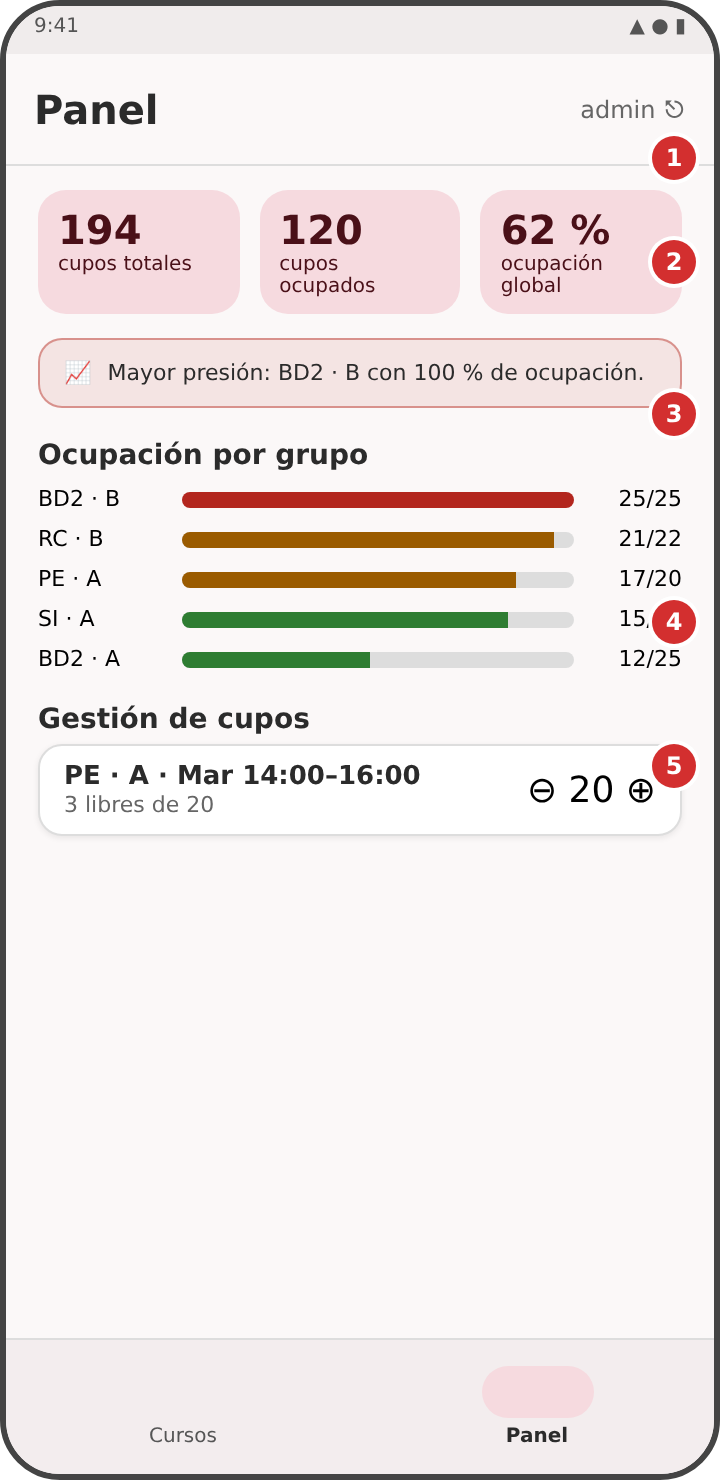
\includegraphics[width=\linewidth]{img/m09_panel.png}\end{minipage}\hfill
\begin{minipage}[c]{0.60\textwidth}\footnotesize\begin{tabularx}{\linewidth}{|c|p{2.3cm}|X|}\hline\rowcolor{tablebackground}\color{white}\textbf{N.°} & \color{white}\textbf{Elemento} & \color{white}\textbf{Widget}\\\hline
1 & Barra superior & \texttt{AppBar} \\\hline
2 & Resúmenes & \texttt{GridView.count(crossAxisCount: 3)} \\\hline
3 & Grupo con mayor presión & \texttt{Aviso} coloreado según el estado del grupo \\\hline
4 & Ocupación por grupo & \texttt{Row}[\texttt{SizedBox(74)}, \texttt{Expanded}(\texttt{LinearProgressIndicator}), \texttt{SizedBox(56)}] \\\hline
5 & Gestión de cupos & \texttt{ListTile} con \texttt{trailing} = \texttt{SizedBox(128)} $\rightarrow$ \texttt{Row}[\texttt{IconButton}, \texttt{Text}, \texttt{IconButton}] \\\hline
\end{tabularx}\end{minipage}
\caption{Mockup: Pestaña Panel (administrador).}\label{fig:m09}\end{figure}


\FloatBarrier
\subsubsection*{Versión para tableta (1000 $\times$ 640 dp)}
Con 600\,dp o más, el \texttt{LayoutBuilder} del \texttt{ShellScreen} reemplaza la barra inferior por un \texttt{NavigationRail} dentro de una \texttt{Row}, y el cuerpo ocupa el resto con \texttt{Expanded}. La cuadrícula de cursos pasa a varias columnas porque cada tarjeta tiene un ancho máximo de 480\,dp.

\begin{figure}[H]\centering
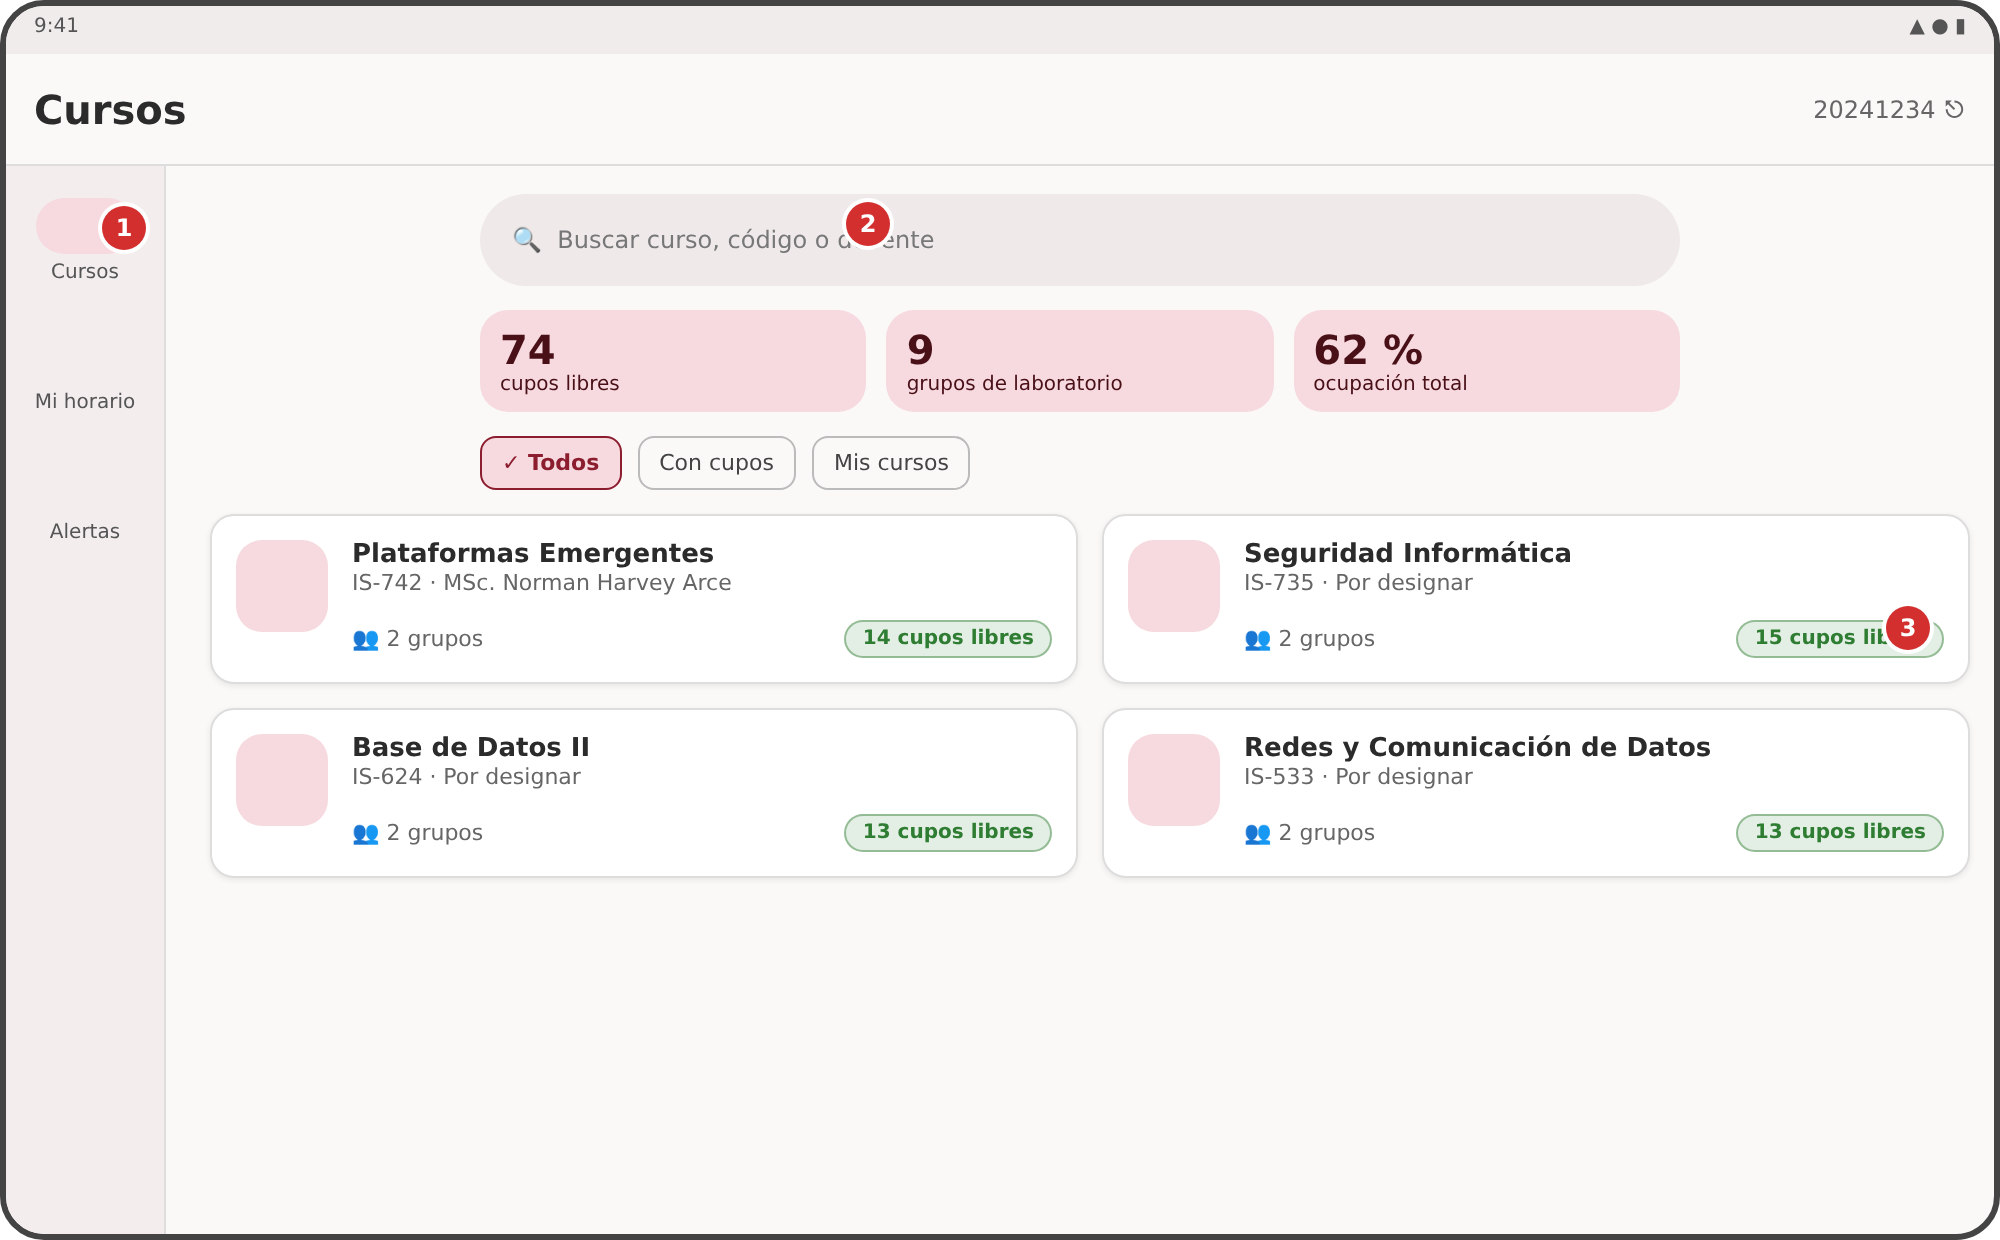
\includegraphics[width=0.95\textwidth]{img/m10_tablet.png}\\[4pt]
\footnotesize\begin{tabularx}{\textwidth}{|c|p{3.6cm}|X|}\hline\rowcolor{tablebackground}\color{white}\textbf{N.°} & \color{white}\textbf{Elemento} & \color{white}\textbf{Widget de Flutter}\\\hline
1 & Riel de navegación & \texttt{Row}[\texttt{NavigationRail}, \texttt{VerticalDivider}, \texttt{Expanded}(cuerpo)] \\\hline
2 & Contenido con ancho máximo & \texttt{ContenidoCentrado(anchoMaximo: 1000)} (\texttt{Align} + \texttt{ConstrainedBox}) \\\hline
3 & Cuadrícula adaptable & \texttt{GridView.builder} con \texttt{SliverGridDelegateWithMaxCrossAxisExtent(480)} \\\hline
\end{tabularx}
\caption{Mockup: Versión para tableta (1000 $\times$ 640 dp).}\label{fig:m10}\end{figure}
